%!TEX program = xelatex
\documentclass[10pt, compress]{beamer}
\usetheme[titleprogressbar]{m}

\usepackage{caption}
\captionsetup[figure]{labelformat=empty}

\usepackage{booktabs}
\usepackage[scale=2]{ccicons}
\usepackage{minted}

\usepgfplotslibrary{dateplot}

\usemintedstyle{trac}

\newcommand{\infbar}{\rule[0.25\baselineskip]{0.5\textwidth}{\linethickness}}

\title{Philosophical Writing in Early New Zealand Newspapers}
\date{\today}
\author{Joshua Black}
\institute{\vspace{30mm}
\includegraphics[width=0.5\textwidth]{images/UC_ARTS_DIGITAL_LAB_2_LINES.png}}

%\setbeamercolor{alerted text}{fg=black}

\begin{document}

\maketitle

\begin{frame}
	\frametitle{Overview}

  \pause

  \begin{enumerate}[<+- | alert@+>]
  \item Problem:
	\begin{itemize}
		\item to gain insight into philosophical writing in early New Zealand newspapers
	\end{itemize}
	\item Method:
	\begin{itemize}
		\item corpus construction via self-labelling and supervised learning,
		\item corpus analysis with, e.g., co-occurrence networks.
	\end{itemize}
	\item Results
	\item Upshot:
	\begin{itemize}
		\item a method applicable for many humanities research questions,
		\item but with shortcomings to be aware of.
	\end{itemize}
	\end{enumerate}

\end{frame}

\section{Problem}

\begin{frame}
	\frametitle{Background}

  \pause

  \begin{itemize}[<+- | alert@+>]
		\item Organisation:
		\begin{itemize}
			\item UC Arts Digital Lab
			\item \ldots part of the digital humanities department.
			\item Digital humanities: use of computational (and data science) techniques to achieve insight into cultural products and practices.
		\end{itemize}
		\item Myself:
		\begin{itemize}
			\item research background in traditional humanities research (in philosophy),
			\item with newly developed data science skills.
 		\end{itemize}
	\end{itemize}

\end{frame}

\begin{frame}
	\frametitle{Humanities Problem}

  \pause

  \begin{itemize}[<+- | alert@+>]
		\item Histories of philosophy in New Zealand don't have much to say before the mid-twentieth century:
			\begin{itemize}
				\item `many of those who had longstanding chairs published next to nothing’ (Davies and Helgeby 2014, 24).
			\end{itemize}
		\item An explanation: excessive on focus academic publications.
		\begin{itemize}
			\item \ldots and on \emph{academic} philosophy.
		\end{itemize}
		\item Newspapers as an alternative source:
		\begin{itemize}
			\item `the fundamental infrastructure for intellectual life \ldots
			\item \ldots newspapers were ascendant in New Zealand because imported books were expensive and a sustainable local periodical literature was slow to emerge' (Ballantyne 2012, 57--78).
			\item Promising: a venue both for the academics and the wider public?
		\end{itemize}
		\item An example of the kind of thing we're after:
	\end{itemize}

\end{frame}

\begin{frame}
	\begin{center}
	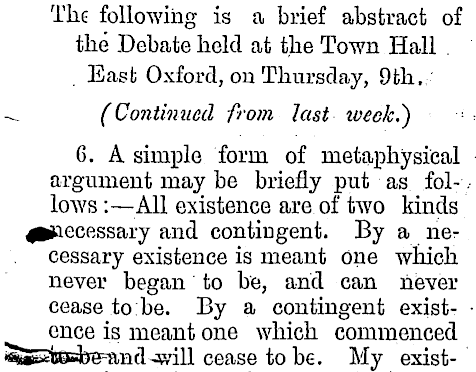
\includegraphics[width=\textwidth]{images/oo.png}
	\end{center}
\end{frame}

\begin{frame}
	\frametitle{Data Science Methods}

  \pause

  \begin{itemize}[<+- | alert@+>]
		\item Data source: the National Library Papers Past Newspaper Open Data Pilot.
		\begin{itemize}
			\item A dataset containing the output of OCR for newspaper data in English up to 1900.
			\item Made available in 2020 to encourage digital experimentation.
			\item `Big' by human standards: 1,471,384 pages of content. (315GB compressed)
			\item Ethics:
			\begin{itemize}
			\item all out of copyright, no living people discussed, but \ldots
			\item some offensive material present.
		\end{itemize}
			\item \url{https://natlib.govt.nz/about-us/open-data/papers-past-metadata/papers-past-newspaper-open-data-pilot/}
		\end{itemize}
		\item Data science methods needed to:
		\begin{itemize}
			\item Find the relevant material (it's a small portion of the data set!)
			\item Derive insight from it once found (it's still a lot of text!)
			\item We will engage in `distant reading' (Moretti 2013)
		\end{itemize}
	\end{itemize}

\end{frame}

\begin{frame}
	\frametitle{The Project}

	\pause

  \begin{enumerate}[<+- | alert@+>]
		\item Corpus construction
		\begin{itemize}
			\item Aim: find the relevant material in the dataset.
			\item Method: labelling articles and training Naive Bayes classifiers following a `bootstrapping' pattern.
		\end{itemize}
		\item Corpus analysis
		\begin{itemize}
			\item Aim: use the corpus to learn something about philosophical writing in NZ newspapers.
			\item Method: many text analysis methods, including concordancing, collocations, co-occurrence networks, and topic modelling.
			\item This presentation will focus on co-occurrence networks.
		\end{itemize}
	\end{enumerate}

\end{frame}

\section{Method}

\begin{frame}
	\frametitle{Corpus Construction Flow Diagram}
	\begin{center}
	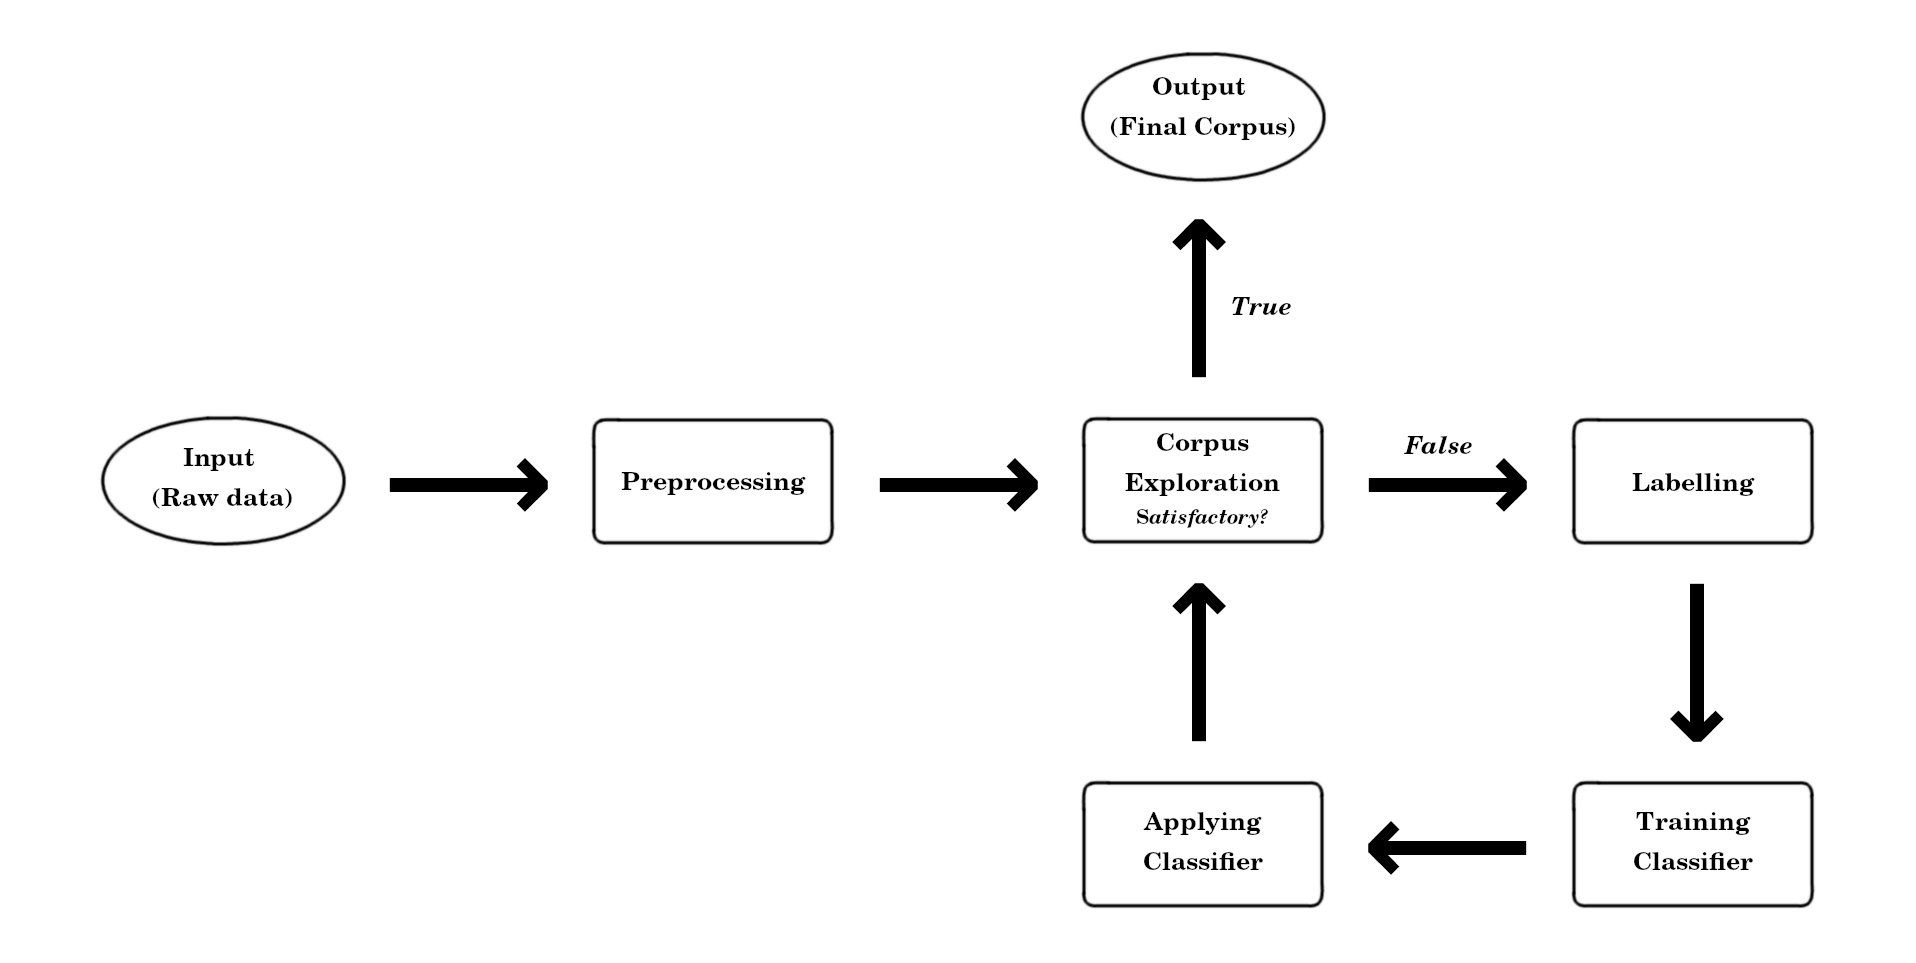
\includegraphics[width=\textwidth]{images/flow_diagram.png}
	\end{center}
\end{frame}

\begin{frame}
	\frametitle{Preprocessing (XML $\rightarrow$ Pandas)}

	\pause

  \begin{itemize}[<+- | alert@+>]
		\item Data format for each issue:
		\begin{itemize}
			\item a METS file with structural information and an ALTO file for each page.
		\end{itemize}
		\item Throw away:
		\begin{itemize}
			\item Spatial information (e.g. location of each word on page)
			\item Items tagged as advertisements.
		\end{itemize}
		\item Method:
		\begin{enumerate}
			\item iterate through title-year tarballs,
			\item for each issue, collect list of articles and corresponding text blocks from METS file,
			\item iterate through ALTO files, collecting text blocks for each article
			\item gather all in Pandas dataframe with each row corresponding to an individual article.
		\end{enumerate}
		\item Result:
		\begin{itemize}
			\item 7,592,619 distinct articles and their plain text,
			\item \ldots stored as eight pickled dataframes (around 8GB total).
		\end{itemize}
	\end{itemize}

\end{frame}

\begin{frame}
	\frametitle{Corpus Construction Flow Diagram}
	\begin{center}
	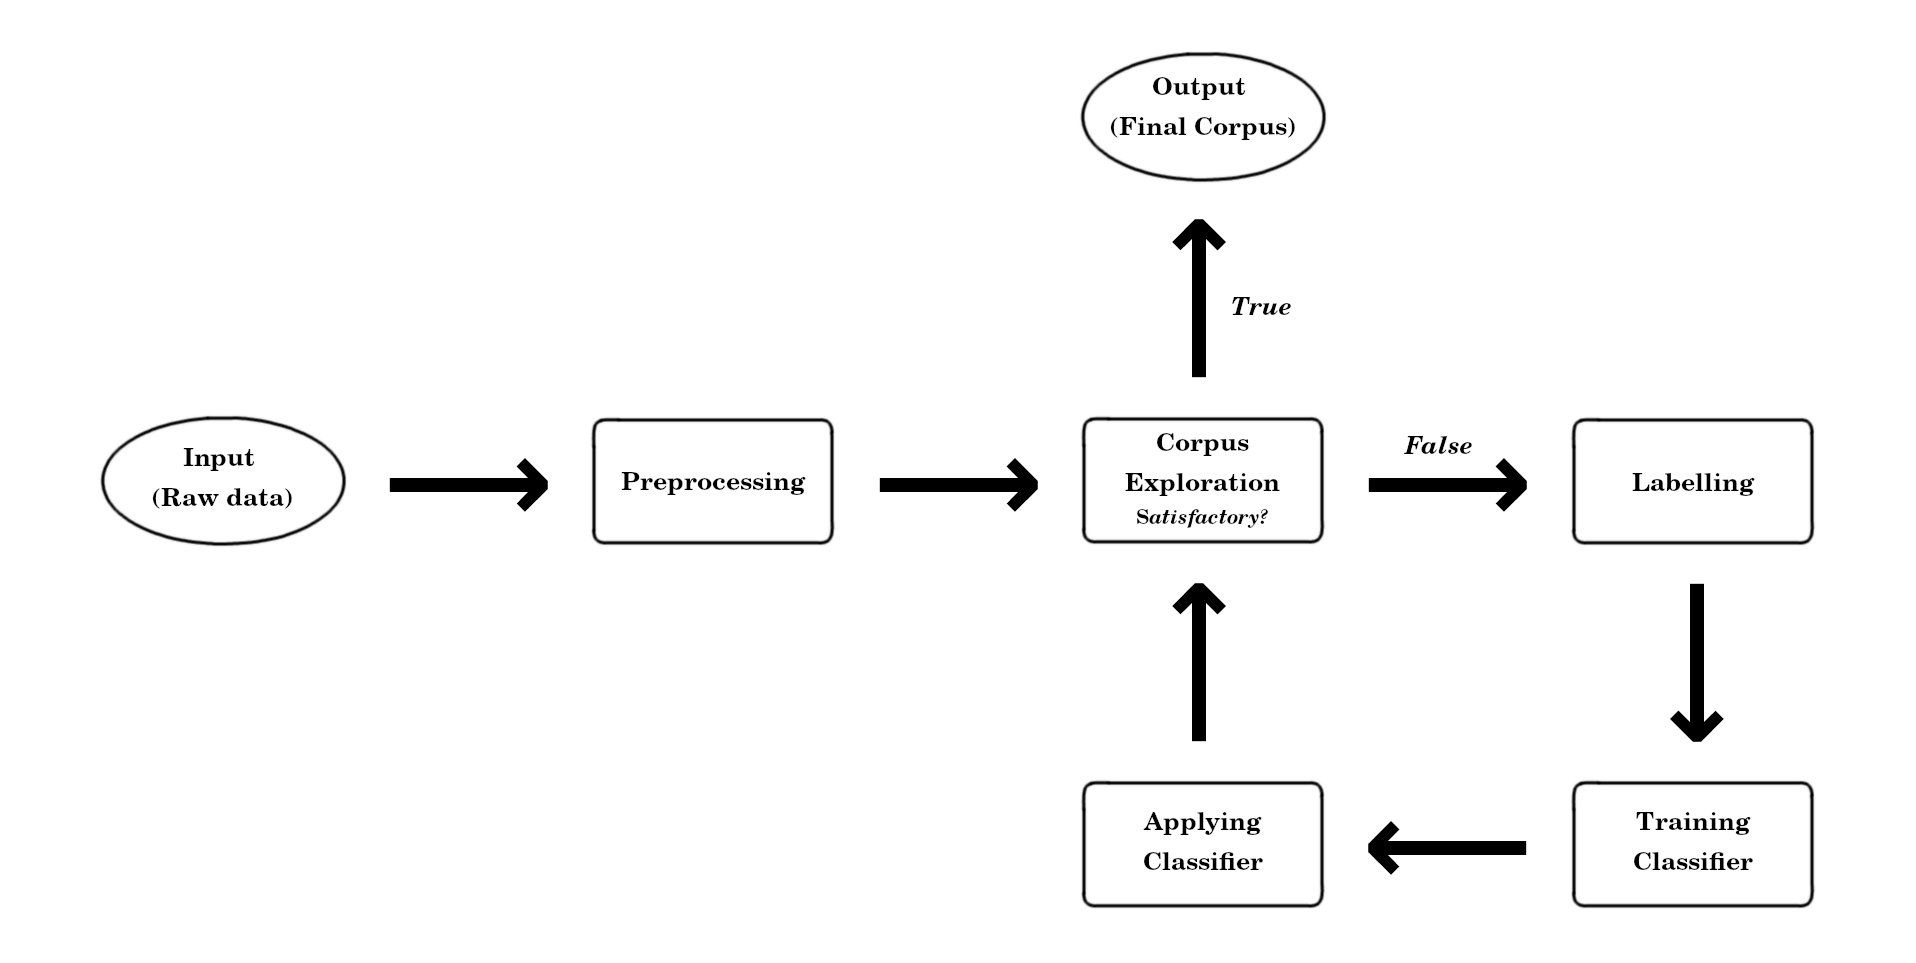
\includegraphics[width=\textwidth]{images/flow_diagram.png}
	\end{center}
\end{frame}

\begin{frame}
	\frametitle{Corpus Exploration}

	\pause

  \begin{itemize}[<+- | alert@+>]
		\item First stage: look at REGEX matched for `philoso*'
		\item Lots of methods used to pick out desired and non-desired articles:
		\begin{itemize}
			\item inspecting random articles, keyword searches, word clounds, concordancing, collocations, co-occurrence networks \ldots
			\item \ldots more on co-occurrence networks later.
		\end{itemize}
		\item If the corpus contains lots of material that we are not interested in, it is not `satisfactory'. If so, we move to the next stage.
	\end{itemize}

\end{frame}

\begin{frame}
	\frametitle{Corpus Construction Flow Diagram}
	\begin{center}
	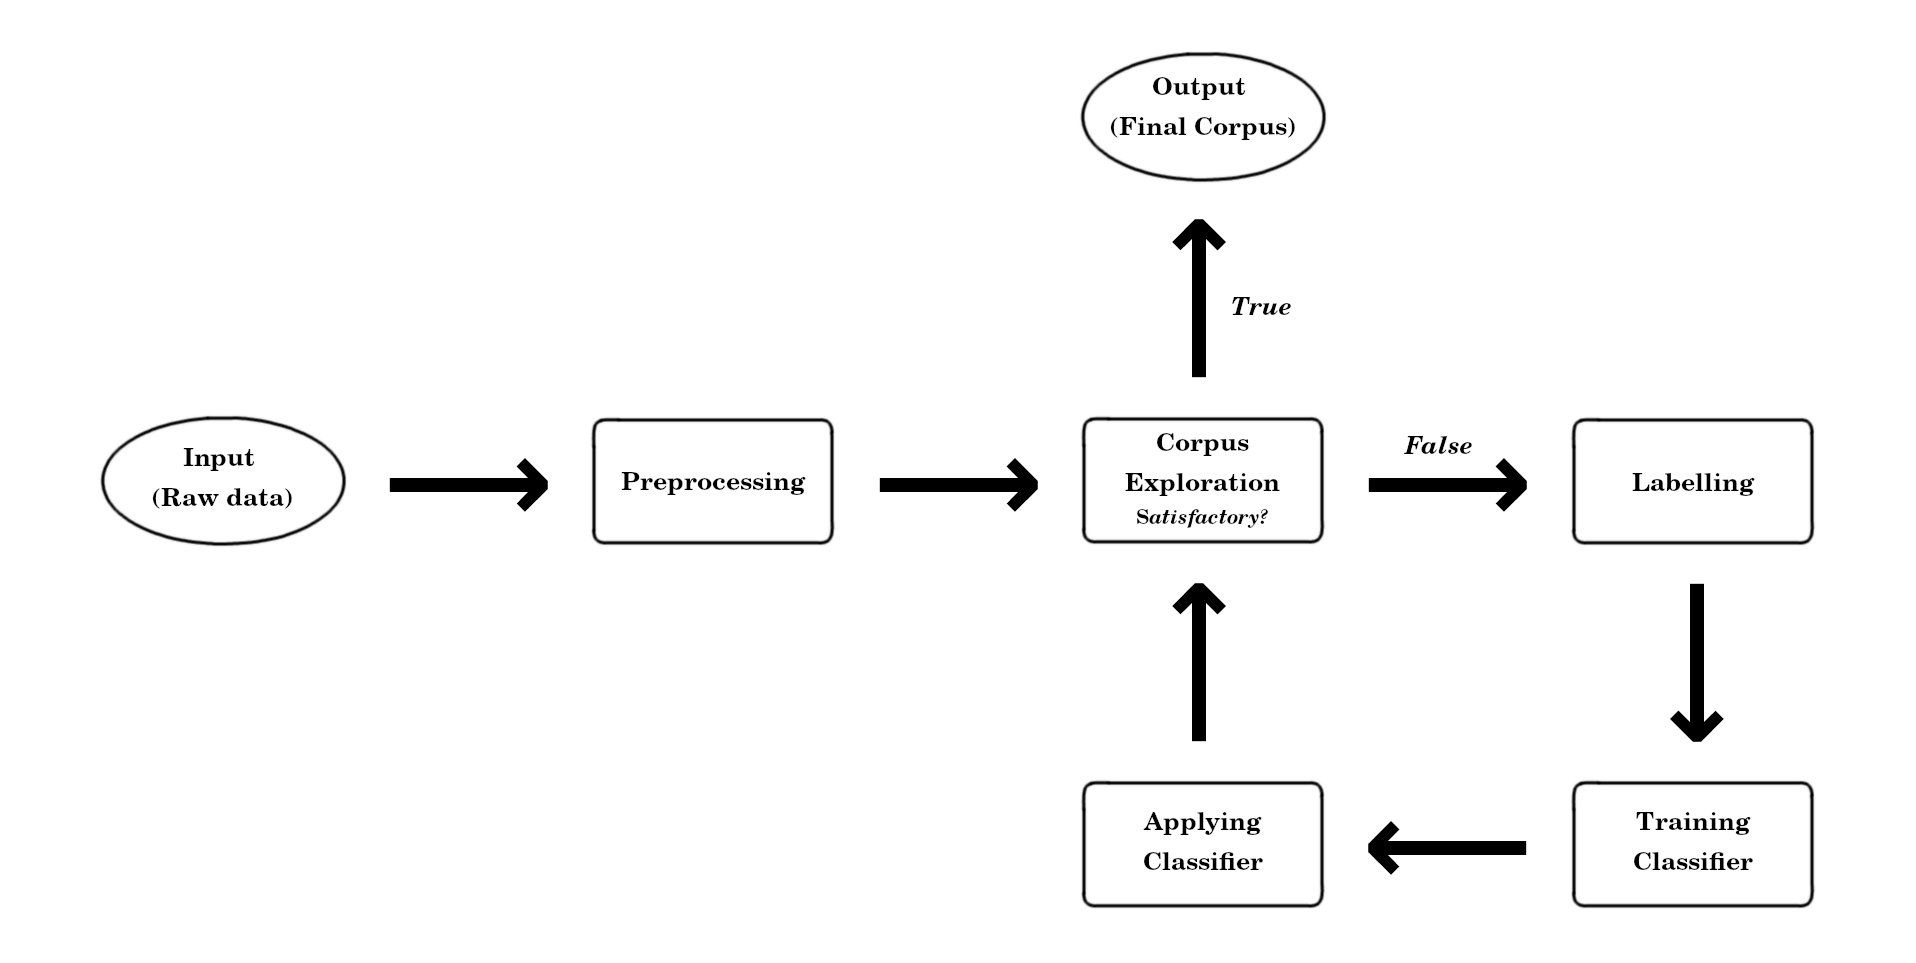
\includegraphics[width=\textwidth]{images/flow_diagram.png}
	\end{center}
\end{frame}

\begin{frame}
	\frametitle{Labelling}

	\pause

  \begin{itemize}[<+- | alert@+>]
		\item Label articles in order to train a classifier to find what we are after.
		\item Two key labels for the project:
		\begin{itemize}
			\item Philosophy: is the majority of the article `philosophical discourse'?
			\begin{itemize}
				\item A broad definition: does it develop or discuss ideas `ultimate reality' or `ultimate value'.
				\item e.g.: is there life after death, are there multiple sources of knowledge, what is the best way to organise society and why?
				\item Some reliance on my own experience in studying 19th century philosophy.
			\end{itemize}
			\item Philosophy type:
			\begin{itemize}
				\item Is it about ethics, the relationship between religious belief and modern thought, metaphysics and epistemology, or other?
				\item The relationship between religious belief and, e.g., evolution is a very prominent topic at this time.
			\end{itemize}
		\item Also attempted, but not used: `Readable', `Writing Type', `NZ author'
		\end{itemize}
		\item NB: it is important to ensure that we label a wide range of non-philosophy.
	\end{itemize}

\end{frame}

\begin{frame}
	\frametitle{Corpus Construction Flow Diagram}
	\begin{center}
	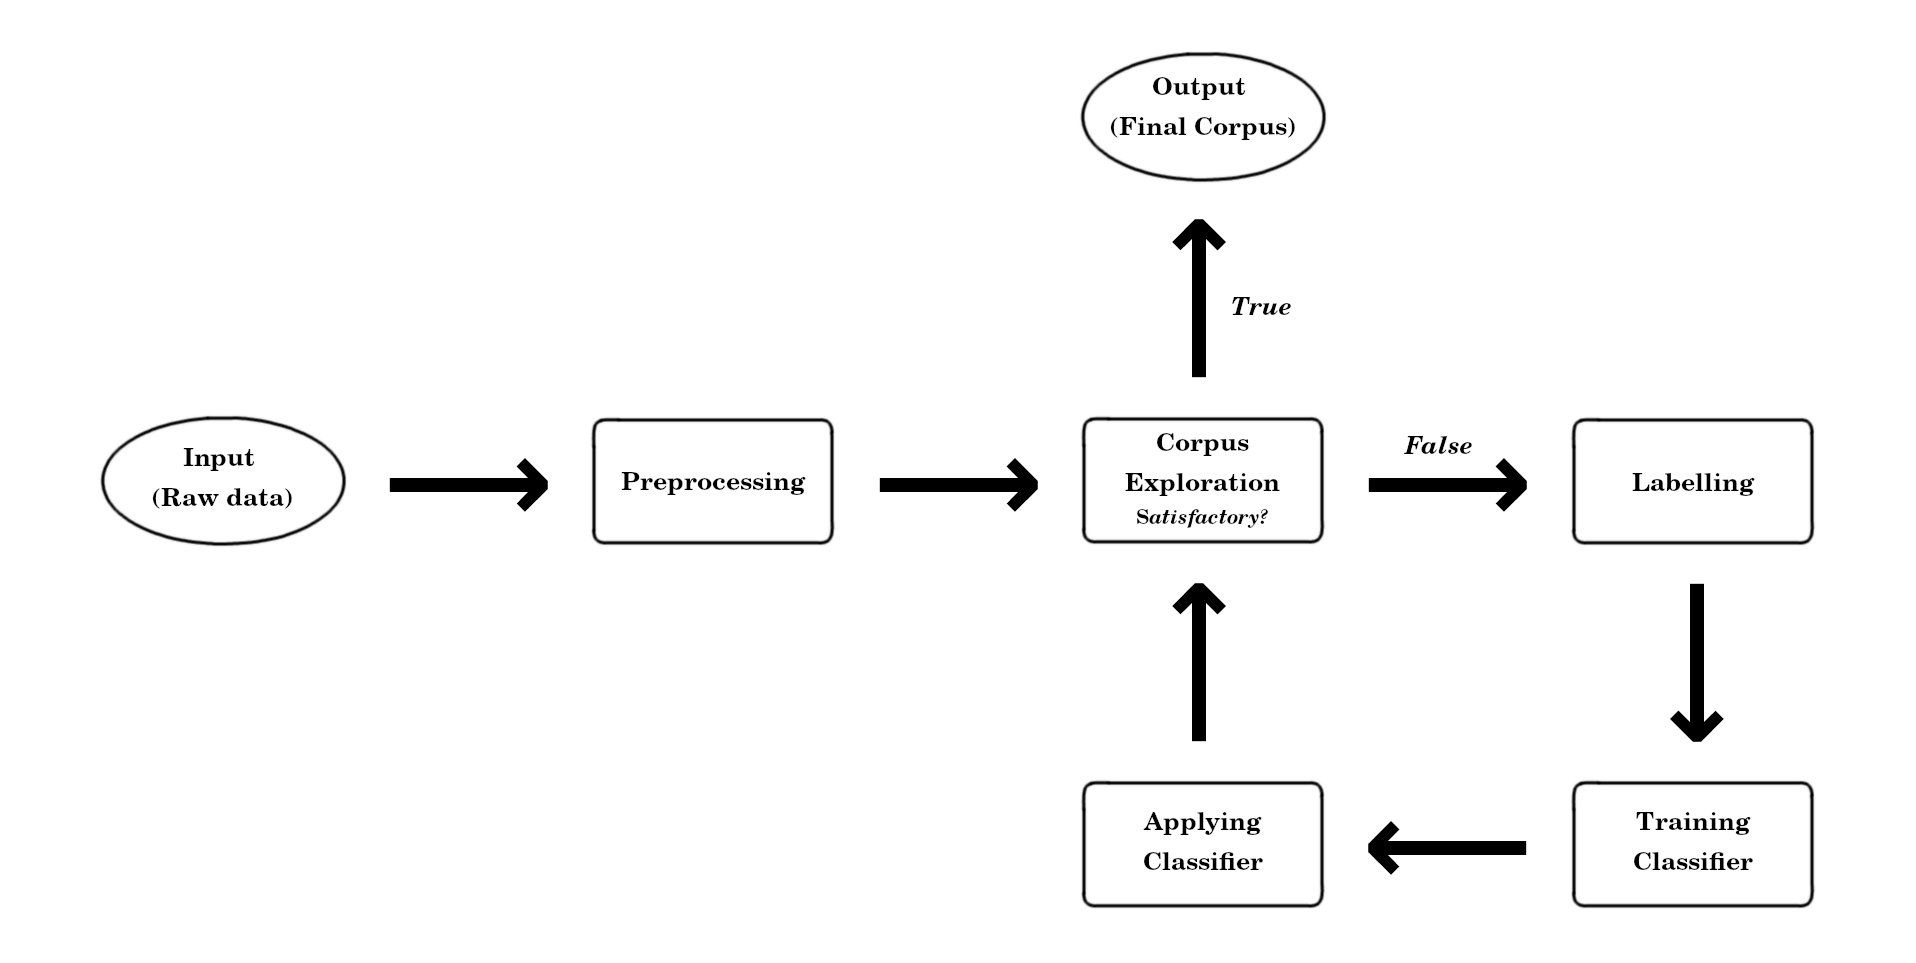
\includegraphics[width=\textwidth]{images/flow_diagram.png}
	\end{center}
\end{frame}

\begin{frame}
	\frametitle{Training and Applying Classifier}

	\pause

  \begin{itemize}[<+- | alert@+>]
		\item Train a classifier to distinguish `philosophy' articles from `non-philosophy'.
		\item Classifiers tried: Naive Bayes and Support Vector Machines
		\item Naive Bayes is simple and fast to train, while performing remarkably effectively.
		\item Training and testing data divided, and training data resampled, as appropriate given the state of the labelled collection.
		\item Classification algorithms mplemented using Scikit-learn Pipelines.
		\begin{enumerate}
			\item Text to bag of words (params: size of feature space)
			\item TF-IDF transformation
			\item The Naive Bayes classifier (params: prior on representativeness of labelled set.)
		\end{enumerate}
		\item Grid CV search used to select parameters for the classifier.
		\item \ldots with accuracy, recall, and precision tried as measures.
		\item Trained classifier applied to complete dataset, treating the `philosophy' articles as a new candidate corpus.
	\end{itemize}

\end{frame}

\begin{frame}
	\frametitle{Corpus Construction Flow Diagram}
	\begin{center}
	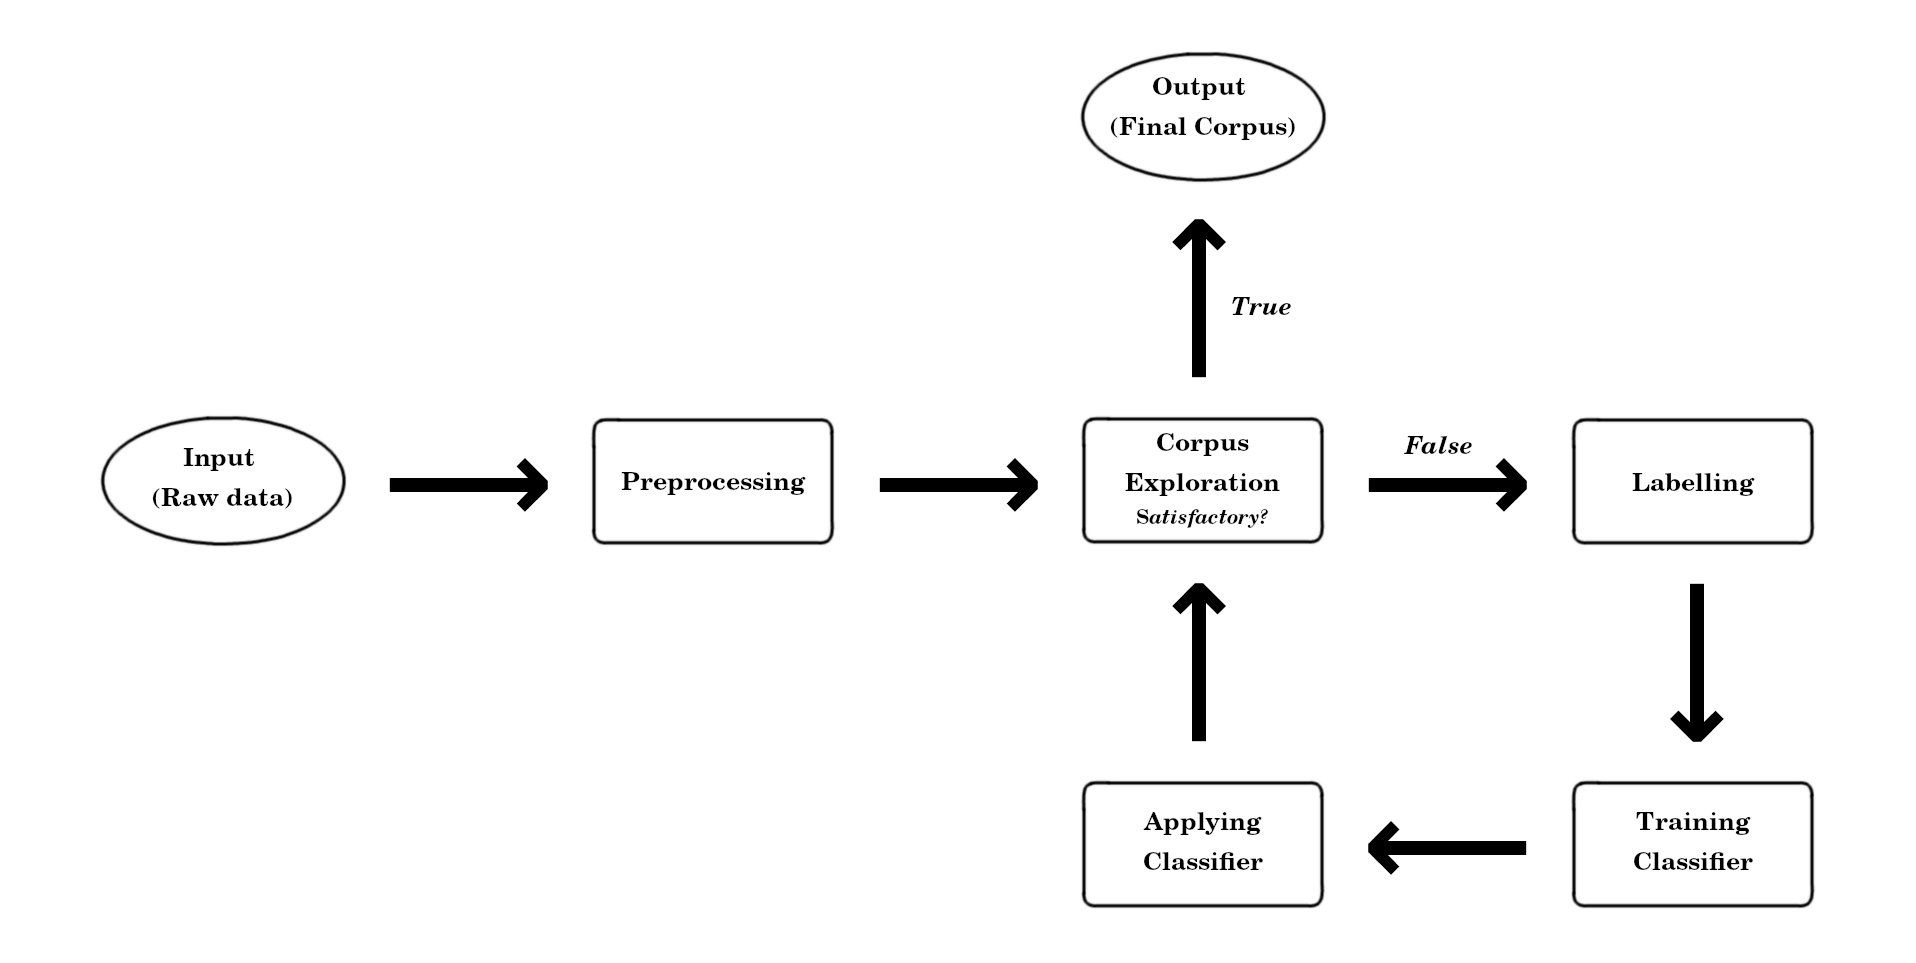
\includegraphics[width=\textwidth]{images/flow_diagram.png}
	\end{center}
\end{frame}

\begin{frame}
	\frametitle{`Bootstrapping'}

	\pause

  \begin{itemize}[<+- | alert@+>]
		\item The phrase: `pull yourself up by the bootstraps',
		\item In this case:
		\begin{enumerate}
			\item starting with nothing, we add articles to our labelled collection,
			\item having collected a good number ($\sim$200-300), with much higher representation of philosophy than the general dataset,
			\item we train and apply a classifier,
			\item we use the articles classifier as philosophy as a source of new articles to label.
		\end{enumerate}
		\item NB: after the first classifier has been applied, the new non-philosophy articles added to the labelled collection will have been classifier as philosophy by the previous classifier.
		\begin{itemize}
		\item \ldots this means that subsequently trained classifiers can be more selective.
		\item \ldots we need a picky classifier.
		\item Stop when satisfied that the corpus does not contain too much `non-philosophy'
		\end{itemize}
	\end{itemize}

\end{frame}

\begin{frame}
	\frametitle{Aim 2: Corpus Analysis}

	\pause

  \begin{itemize}[<+- | alert@+>]
		\item Corpus analysis $\sim$ the corpus exploration step.
		\item One method used: co-occurrence networks:
		\begin{enumerate}
			\item create bag or words or TF-IDF representation of documents;
			\item compute a document-term matrix (num terms x num documents) for either the BOW or TF-IDF representation;
			\item compute a term-term matrix (num terms x num terms), representing co-occurrences in documents of each pair of terms; and
			\item given a search term, pass these matrices to a statistical function to return the most closely related words.
			\begin{itemize}
				\item Statistics implemented: log Dice and mutual information.
			\end{itemize}
		\end{enumerate}
		\item Networks displayed using Dash cytoscapes:
		\begin{itemize}
		\item see project dashboard: \url{nz-newspaper-philosophy.herokuapp.com}
		\end{itemize}
		\item NB: term-term matrices can get very large. Various methods to control the size of the dictionary were employed.
	\end{itemize}

\end{frame}

\section{Results}

\begin{frame}
	\frametitle{Corpus Construction (Size Reduction)}

	\pause

	Classifiers become more selective:

	\begin{table}[]
	        \centering
	        \begin{tabular}{l|c}
	             Corpus &  Article Count \\
	             \hline
						Processed dataset & 7592619 \\
	        	(Step 0) `philoso*' Corpus &	29647 \\
	        	(Step 1) Naive Bayes 1 &	239649 \\
	          (Step 2) Naive Bayes 2 & 31131
	        \end{tabular}
	        \caption{Article counts for processed dataset and general philosophy corpora.}
	        \label{t:corpus-sizes}
	\end{table}

\end{frame}

\begin{frame}
	\frametitle{Word Cloud: Sample of Processed Dataset}
	\begin{center}
		
\includegraphics[width=\textwidth]{images/corpus_10000_subset_tf-idf.png}
	\end{center}
\end{frame}

\begin{frame}
	\frametitle{Word Cloud: Step 0}
	\begin{center}
		
\includegraphics[width=\textwidth]{images/philoso_tf-idf.png}
	\end{center}
\end{frame}

\begin{frame}
	\frametitle{Word Cloud: Step 1}
	\begin{center}
		
\includegraphics[width=\textwidth]{images/nb1_philoso_tf-idf.png}
	\end{center}
\end{frame}

\begin{frame}
	\frametitle{Word Cloud: Step 2}
	\begin{center}
		
\includegraphics[width=\textwidth]{images/nb2_v2_philoso_tf-idf.png}
	\end{center}
\end{frame}

\begin{frame}
	\frametitle{Labelling}

	\begin{table}[]
	        \centering
	        \scriptsize
	        \begin{tabular}{l|ll|ll}
	          & \textbf{Step 1} & & \textbf{Step 2}  & \\
	          Label & Value & Count & Value & Count \\
	          \hline
	          & & & &  \\
	        	Readable & True & 247 & True & 918 \\
	        	& False & 26 & False & 41 \\
	          & & & &  \\
	          Philosophy & True & 101 & True & 299 \\
	          & False & 147 & False & 620 \\
	          & & & &  \\
	          Philosophy Type & Religion-Science & 58 & Religion-Science & 140 \\
	          & Ethics-Politics & 25 &  Ethics-Politics & 94 \\
	          & Epistemology-Metaphysics & 3 & Epistemology-Metaphysics & 13 \\
	          & Other & 15 &  Other & 52 \\
	          & & & &  \\
	          Writing Type & Public Event & 40 & Public Event & 97 \\
	          & Letter to the Editor & 23 &  Letter to the Editor & 69 \\
	          & First-order Writing & 36 &  First-order Writing & 111 \\
	          & Review & 2 &  Other & 22 \\
	          & & & &  \\
	          NZ & True & 77 & True & 178 \\
	          & False & 12 & False & 41 \\
	        \end{tabular}
	        \caption{Label counts at Step 1 and Step 2.}
	        \label{t:labels}
	\end{table}
\end{frame}

\begin{frame}
	\frametitle{Classifier Performance (Step 2)}

	\pause
	\begin{table}[]
	        \centering
	        \footnotesize
	        \begin{tabular}{ll|ll}
	        & & \textbf{Predicted} & \\
	        & & False & True \\
	        \hline
	        \textbf{Actual} & False & 181 & 14 \\
	        & True & 15 & 62 \\
	        \end{tabular}
	        \caption{Confusion Matrix for Second Naive Bayes Classifier}
	        \label{t:nb2-confusion}
	\end{table}

	\begin{itemize}
		\item Accuracy: 0.89
		\item Precision: 0.81
		\item Recall: 0.80
	\end{itemize}
\end{frame}

\begin{frame}
	\frametitle{Corpus Performance}

	\pause

  \begin{itemize}[<+- | alert@+>]
		\item Metrics are not bad, but not great either.
		\item Inspection of the false positives and negatives reveals:
		\begin{itemize}
			\item prevalence of `composite articles' in the false negatives, where only one or two bits are philosophical; and
			\item prevalence of `edge cases' and mistaken labelling in the false positives.
		\end{itemize}
		\item Conclusion: the performance of the classifiers is being limited by the quality of the labels.
	\end{itemize}

\end{frame}

\begin{frame}
	\frametitle{Corpus Analysis}

	\pause

  \begin{itemize}[<+- | alert@+>]
		\item Many methods were used at this stage (see project report)
		\item The following two slides contain:
		\begin{enumerate}
			\item an example of a telling co-occurrence network, and
			\item a choropleth revealing prominence of religion and science discourse in different regions.
		\end{enumerate}
	\end{itemize}

\end{frame}

\begin{frame}
	\begin{center}
		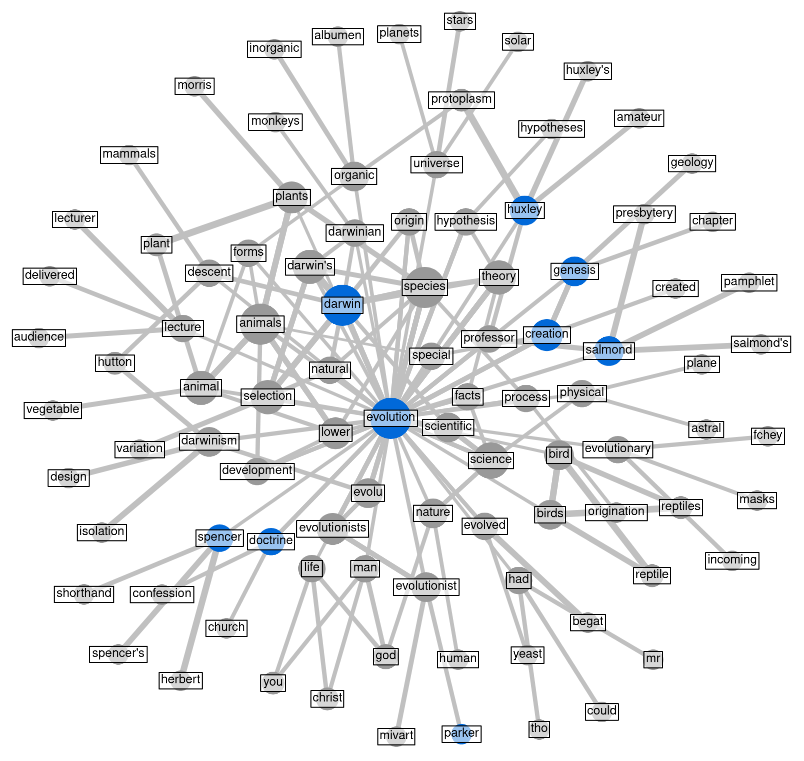
\includegraphics[width=0.9\textwidth]{images/evo_net.png}
	\end{center}

\end{frame}

\begin{frame}
	\begin{center}
		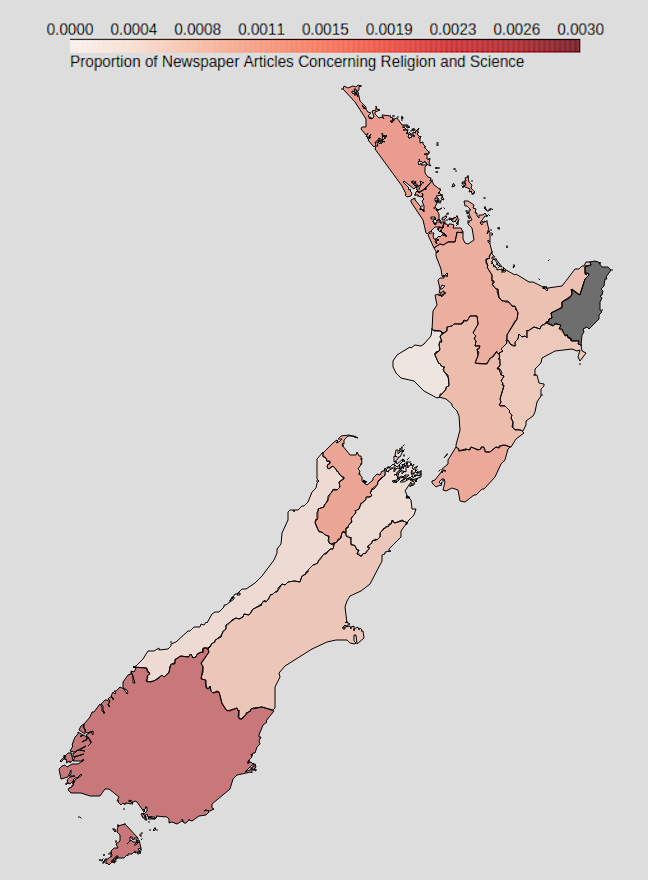
\includegraphics[width=0.6\textwidth]{images/choropleth.png}
	\end{center}

\end{frame}


\section{Upshot}


\begin{frame}
	\frametitle{Positives}

	\pause

  \begin{enumerate}[<+- | alert@+>]
		\item Single investigator, self-labelled corpus production using METS/ALTO digitised newspaper files is feasible.
		\begin{itemize}
			\item Generalisability: METS/ALTO is the standard for newspaper digitisation, so the same methods could be applied in other countries.
		\end{itemize}
		\item The corpus produced at the corpus construction stage shows potential for research into early New Zealand philosophy.
	\end{enumerate}

\end{frame}

\begin{frame}
	\frametitle{Shortcomings}

	\pause

  \begin{enumerate}[<+- | alert@+>]
		\item Problem 1:
		\begin{itemize}
		\item Many articles at the time were made up of lots of distinct bits (especially editorials).
		\item Since the classifier loses many of these articles, the resulting corpus is not fully representative of philosophical discourse in early NZ newspapers.
		\item Possible solution: label text blocks rather than articles.
	\end{itemize}
	\item Problem 2:
		\begin{itemize}
			\item Labelling criteria were insufficiently clear.
			\item Better labelling might improve classifier performance.
			\item Possible alternative: start with easier distinctions (e.g. is the article a report of a public lecture?), then move to subject matter distinctions.
		\end{itemize}
	\end{enumerate}

\end{frame}

\begin{frame}
	\frametitle{Overview}

  \pause

  \begin{enumerate}[<+- | alert@+>]
  \item Problem:
	\begin{itemize}
		\item to gain insight into philosophical writing in early New Zealand newspapers
	\end{itemize}
	\item Method:
	\begin{itemize}
		\item corpus construction via self-labelling and supervised learning,
		\item corpus analysis with, e.g., co-occurrence networks.
	\end{itemize}
	\item Results:
	\begin{itemize}
		\item An interesting collection of articles for digital humanities research,
		\item with indications that labelling could be improved,
		\item and ability to reveal features of philosophical discourse about relationship between religious belief and then-new scientific ideas.
	\end{itemize}
	\item Upshot:
	\begin{itemize}
		\item a method applicable for many humanities research questions,
		\item but with shortcomings to be aware of.
	\end{itemize}
	\end{enumerate}

\end{frame}

\begin{frame}
	\frametitle{Links}

  \begin{itemize}
		\item Dashboard: \url{nz-newspaper-philosophy.herokuapp.com}
		\item GitHub (full project): \url{github.com/JoshuaDavidBlack/NPOD_Philosophy}
		\item GitHub (dashboard): \url{github.com/JoshuaDavidBlack/NPOD_Philosophy_Heroku}
	\end{itemize}

\end{frame}


\end{document}
